\ifx\allfiles\undefined
\documentclass[12pt, a4paper, oneside, UTF8]{ctexbook}
\def\path{../config}
\usepackage{amsmath}
\usepackage{amsthm}
\usepackage{array}
\usepackage{amssymb}
\usepackage{graphicx}
\usepackage{mathrsfs}
\usepackage{enumitem}
\usepackage{geometry}
\usepackage[colorlinks, linkcolor=black]{hyperref}
\usepackage{stackengine}
\usepackage{yhmath}
\usepackage{extarrows}
% \usepackage{unicode-math}
\usepackage{esint}
\usepackage{multirow}
\usepackage{fancyhdr}
\usepackage[dvipsnames, svgnames]{xcolor}
\usepackage{listings}
\usepackage{float} % Required for the H float option
\definecolor{mygreen}{rgb}{0,0.6,0}
\definecolor{mygray}{rgb}{0.5,0.5,0.5}
\definecolor{mymauve}{rgb}{0.58,0,0.82}
\definecolor{NavyBlue}{RGB}{0,0,128}
\definecolor{Rhodamine}{RGB}{255,0,255}
\definecolor{PineGreen}{RGB}{0,128,0}

\graphicspath{ {figures/},{../figures/}, {config/}, {../config/} }

\linespread{1.6}

\geometry{
    top=25.4mm, 
    bottom=25.4mm, 
    left=20mm, 
    right=20mm, 
    headheight=2.17cm, 
    headsep=4mm, 
    footskip=12mm
}

\setenumerate[1]{itemsep=5pt,partopsep=0pt,parsep=\parskip,topsep=5pt}
\setitemize[1]{itemsep=5pt,partopsep=0pt,parsep=\parskip,topsep=5pt}
\setdescription{itemsep=5pt,partopsep=0pt,parsep=\parskip,topsep=5pt}

\lstset{
    language=Mathematica,
    basicstyle=\tt,
    breaklines=true,
    keywordstyle=\bfseries\color{NavyBlue}, 
    emphstyle=\bfseries\color{Rhodamine},
    commentstyle=\itshape\color{black!50!white}, 
    stringstyle=\bfseries\color{PineGreen!90!black},
    columns=flexible,
    numbers=left,
    numberstyle=\footnotesize,
    frame=tb,
    breakatwhitespace=false,
} 

\lstset{
    language=TeX, % 设置语言为 TeX
    basicstyle=\ttfamily, % 使用等宽字体
    breaklines=true, % 自动换行
    keywordstyle=\bfseries\color{NavyBlue}, % 关键字样式
    emphstyle=\bfseries\color{Rhodamine}, % 强调样式
    commentstyle=\itshape\color{black!50!white}, % 注释样式
    stringstyle=\bfseries\color{PineGreen!90!black}, % 字符串样式
    columns=flexible, % 列的灵活性
    numbers=left, % 行号在左侧
    numberstyle=\footnotesize, % 行号字体大小
    frame=tb, % 顶部和底部边框
    breakatwhitespace=false % 不在空白处断行
}

% \begin{lstlisting}[language=TeX] ... \end{lstlisting}

% 定理环境设置
\usepackage[strict]{changepage} 
\usepackage{framed}

\definecolor{greenshade}{rgb}{0.90,1,0.92}
\definecolor{redshade}{rgb}{1.00,0.88,0.88}
\definecolor{brownshade}{rgb}{0.99,0.95,0.9}
\definecolor{lilacshade}{rgb}{0.95,0.93,0.98}
\definecolor{orangeshade}{rgb}{1.00,0.88,0.82}
\definecolor{lightblueshade}{rgb}{0.8,0.92,1}
\definecolor{purple}{rgb}{0.81,0.85,1}

\theoremstyle{definition}
\newtheorem{myDefn}{\indent Definition}[section]
\newtheorem{myLemma}{\indent Lemma}[section]
\newtheorem{myThm}[myLemma]{\indent Theorem}
\newtheorem{myCorollary}[myLemma]{\indent Corollary}
\newtheorem{myCriterion}[myLemma]{\indent Criterion}
\newtheorem*{myRemark}{\indent Remark}
\newtheorem{myProposition}{\indent Proposition}[section]

\newenvironment{formal}[2][]{%
	\def\FrameCommand{%
		\hspace{1pt}%
		{\color{#1}\vrule width 2pt}%
		{\color{#2}\vrule width 4pt}%
		\colorbox{#2}%
	}%
	\MakeFramed{\advance\hsize-\width\FrameRestore}%
	\noindent\hspace{-4.55pt}%
	\begin{adjustwidth}{}{7pt}\vspace{2pt}\vspace{2pt}}{%
		\vspace{2pt}\end{adjustwidth}\endMakeFramed%
}

\newenvironment{definition}{\vspace{-\baselineskip * 2 / 3}%
	\begin{formal}[Green]{greenshade}\vspace{-\baselineskip * 4 / 5}\begin{myDefn}}
	{\end{myDefn}\end{formal}\vspace{-\baselineskip * 2 / 3}}

\newenvironment{theorem}{\vspace{-\baselineskip * 2 / 3}%
	\begin{formal}[LightSkyBlue]{lightblueshade}\vspace{-\baselineskip * 4 / 5}\begin{myThm}}%
	{\end{myThm}\end{formal}\vspace{-\baselineskip * 2 / 3}}

\newenvironment{lemma}{\vspace{-\baselineskip * 2 / 3}%
	\begin{formal}[Plum]{lilacshade}\vspace{-\baselineskip * 4 / 5}\begin{myLemma}}%
	{\end{myLemma}\end{formal}\vspace{-\baselineskip * 2 / 3}}

\newenvironment{corollary}{\vspace{-\baselineskip * 2 / 3}%
	\begin{formal}[BurlyWood]{brownshade}\vspace{-\baselineskip * 4 / 5}\begin{myCorollary}}%
	{\end{myCorollary}\end{formal}\vspace{-\baselineskip * 2 / 3}}

\newenvironment{criterion}{\vspace{-\baselineskip * 2 / 3}%
	\begin{formal}[DarkOrange]{orangeshade}\vspace{-\baselineskip * 4 / 5}\begin{myCriterion}}%
	{\end{myCriterion}\end{formal}\vspace{-\baselineskip * 2 / 3}}
	

\newenvironment{remark}{\vspace{-\baselineskip * 2 / 3}%
	\begin{formal}[LightCoral]{redshade}\vspace{-\baselineskip * 4 / 5}\begin{myRemark}}%
	{\end{myRemark}\end{formal}\vspace{-\baselineskip * 2 / 3}}

\newenvironment{proposition}{\vspace{-\baselineskip * 2 / 3}%
	\begin{formal}[RoyalPurple]{purple}\vspace{-\baselineskip * 4 / 5}\begin{myProposition}}%
	{\end{myProposition}\end{formal}\vspace{-\baselineskip * 2 / 3}}


\newtheorem{example}{\indent \color{SeaGreen}{Example}}[section]
\renewcommand{\proofname}{\indent\textbf{\textcolor{TealBlue}{Proof}}}
\newenvironment{solution}{\begin{proof}[\indent\textbf{\textcolor{TealBlue}{Solution}}]}{\end{proof}}

% 自定义命令的文件

\def\d{\mathrm{d}}
\def\R{\mathbb{R}}
%\newcommand{\bs}[1]{\boldsymbol{#1}}
%\newcommand{\ora}[1]{\overrightarrow{#1}}
\newcommand{\myspace}[1]{\par\vspace{#1\baselineskip}}
\newcommand{\xrowht}[2][0]{\addstackgap[.5\dimexpr#2\relax]{\vphantom{#1}}}
\newenvironment{mycases}[1][1]{\linespread{#1} \selectfont \begin{cases}}{\end{cases}}
\newenvironment{myvmatrix}[1][1]{\linespread{#1} \selectfont \begin{vmatrix}}{\end{vmatrix}}
\newcommand{\tabincell}[2]{\begin{tabular}{@{}#1@{}}#2\end{tabular}}
\newcommand{\pll}{\kern 0.56em/\kern -0.8em /\kern 0.56em}
\newcommand{\dive}[1][F]{\mathrm{div}\;\boldsymbol{#1}}
\newcommand{\rotn}[1][A]{\mathrm{rot}\;\boldsymbol{#1}}

% 修改参数改变封面样式,0 默认原始封面、内置其他1、2、3种封面样式
\def\myIndex{0}


\ifnum\myIndex>0
    \input{\path/cover_package_\myIndex}
\fi

\def\myTitle{标题:一份LaTeX笔记模板}
\def\myAuthor{作者名称}
\def\myDateCover{封面日期: \today}
\def\myDateForeword{前言页显示日期: \today}
\def\myForeword{前言标题}
\def\myForewordText{
    
    这是一个基于\LaTeX{}的模板,用于撰写学习笔记。

    模板旨在提供一个简单、易用的框架,以便你能够专注于内容,而不是排版细节,如不是专业者,不建议使用者在模板细节上花费太多时间,而是直接使用模板进行笔记撰写。遇到问题,再进行调整解决。
}
\def\mySubheading{副标题}


\begin{document}
% \input{\path/cover_text_\myIndex.tex}

\newpage
\thispagestyle{empty}
\begin{center}
    \Huge\textbf{\myForeword}
\end{center}
\myForewordText
\begin{flushright}
    \begin{tabular}{c}
        \myDateForeword
    \end{tabular}
\end{flushright}

\newpage
\pagestyle{plain}
\setcounter{page}{1}
\pagenumbering{Roman}
\tableofcontents

\newpage
\pagenumbering{arabic}
\setcounter{chapter}{-1}
\setcounter{page}{1}

\pagestyle{fancy}
\fancyfoot[C]{\thepage}
\renewcommand{\headrulewidth}{0.4pt}
\renewcommand{\footrulewidth}{0pt}








\else
\fi

\chapter{可靠度设计原理}

\begin{definition}
    抗力: 结构或构件抵抗外部荷载作用的能力,通常用抗力$R$表示。

    荷载: 包括内力、变形和加速度,通常用载荷$S$表示。
\end{definition}

\begin{example}
    荷载只包括结构的内力(F)

    实际上荷载还包括变形与加速度(小测题)
\end{example}

\section{平稳二项随机过程荷载模型}

\paragraph{基本假定(课后习题考了):}

\begin{enumerate}
    \item 根据荷载每变动一次作用在结构上的时间长短,将设计基准期 \( T \) 等分为 \( r \) 个相等的时段 \( \tau \),或认为设计基准期 \( T \) 内荷载均匀变动 \( r = T / \tau \) 次;

    \item 每一时段 \( \tau \) 内,荷载 \( Q \) 出现(即 \( Q > 0 \))的概率为 \( p \),不出现(即 \( Q = 0 \))的概率为 \( q = 1 - p \);

    \item 每一时段 \( \tau \) 内,荷载出现时,其幅值为非负的随机变量,且在不同时段上的概率分布是相同的,记时段 \( \tau \) 内的荷载概率分布(也称为任意时点荷载分布)为 \( F_i(x) = P[Q(t) \leq x, t \in \tau] \);

    \item 不同时段 \( \tau \) 上荷载幅值随机变量相互独立,且与在时段 \( \tau \) 上是否出现荷载无关。
\end{enumerate}

\begin{figure}[H]
    \centering
    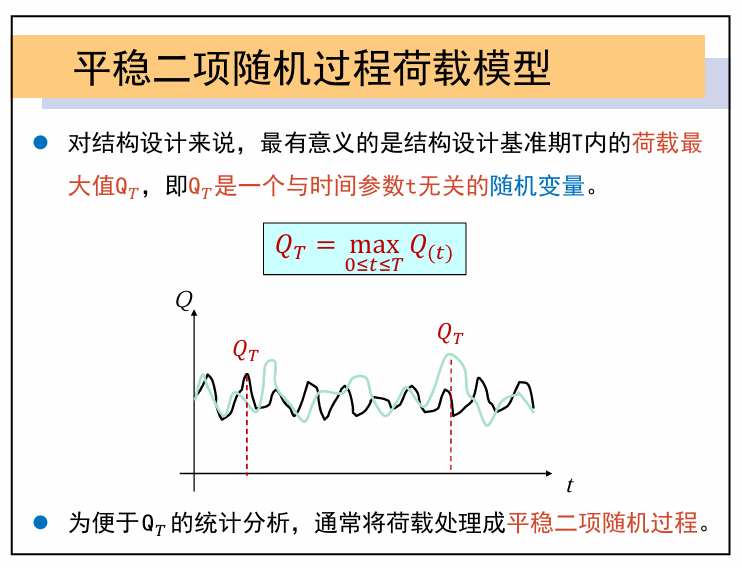
\includegraphics[width=0.6\textwidth]{../figure/pwex.png}
    \caption{平稳二项随机过程荷载模型示意图}
    \label{fig:chap5:fig1}
\end{figure}

\begin{remark}
    此处省略一堆推导,我感觉课本上的推导有些奇怪,概统都是把等于0和小于等于t的分布函数放在一起处理的
\end{remark}

荷载标准值$Q_k$可以定义为在结构设计基准期$T$中具有不被超越的概率$p_k$

永久荷载标准值一般相当于永久荷载概率分布的50\%分位值,即正态分布的平均值

可变荷载(含短时荷载和持久荷载,但都是可变的)标准值是由设计基准期内荷载最大值概率分布的某一个分位值确定的。

\begin{example}
    对于永久荷载,只有一个指标,就是标准值。(T)
\end{example}

\begin{corollary}
    对于可变荷载,有三个指标,准永久值<频遇值<标准值

    这里是按超过该设计值所占的比例从小到大排序的。
    
    比如准永久值是50\%分位值,频遇值是95\%分位值,标准值是99\%分位值。
\end{corollary}

\section{Turkstra组合规则}

\begin{theorem}
    依次将一个荷载效应在设计基准期内的最大值与其余荷载的任意时点值相组合,即
\[
S_{Ci} = \max_{t \in [0, T]} s_i(t) + s_1(t_0) + \cdots + s_{i-1}(t_0) + s_{i+1}(t_0) + \cdots + s_n(t_0)
\]
\[
i = 1, 2, \ldots, n 
\]
式中 \( t_0 \) —— \( s_i(t) \) 达到最大的时刻。
在时间 \( T \) 内,荷载效应组合的最大值 \( S_C \) 取为上列诸组合的最大值,即
\[
S_C = \max(S_{C1}, S_{C2}, \ldots, S_{Cn}) 
\]
其中任一组组合的概率分布,可以根据式中求和项的概率分布通过卷积运算得到。
\end{theorem}

\begin{remark}
    有n个可变荷载时,荷载效应组合的最大值是n个荷载效应组合的最大值。

    但是显然这样不一定就是最差的情况(荷载最大),因为可能n个荷载都不是最大时,总和最大。
\end{remark}


\begin{example}
    Turkstra组合规则考虑了所有可能的最不利荷载组合。(F,如前文所示)

一般情况下,JCSS组合规则考虑的最不利荷载组合数量多于Turkstra组合规则。($2^{n-1} \ge n$)
\end{example}

\section{JCSS组合规则}

\begin{theorem}
    先假定可变荷载的样本函数为平稳二项过程,将某一可变荷载$Q1(t)$在基准期内的最大效应值$maxS1(t)$(持续时间$\tau_1$),与另一可变荷载$Q2(t)$在$\tau_1$内的局部最大效应值$maxS2(t)$(持续时间$\tau_2$),与第三个可变荷载$Q3(t)$在$\tau_2$内的局部最大效应值$maxS3(t)$相组合,以此类推。
\end{theorem}

\begin{remark}
    我是真没看懂教材那里的描述,如果按这样取,那不应该是$n!$项吗?
\end{remark}

\section{抗力}

\begin{definition}
    结构抗力分四个层次:

    \begin{enumerate}
        \item 整体结构抗力(如整体结构承受风荷载的能力)
        \item 结构构件抗力(如构件在轴力、弯矩作用下的承载能力)
        \item 构件截面抗力(构件截面抗弯、抗剪的能力)
        \item 截面各点的抗力(截面各点抵抗正应力、剪应力的能力)
    \end{enumerate}
\end{definition}

\begin{figure}[H]
    \centering
    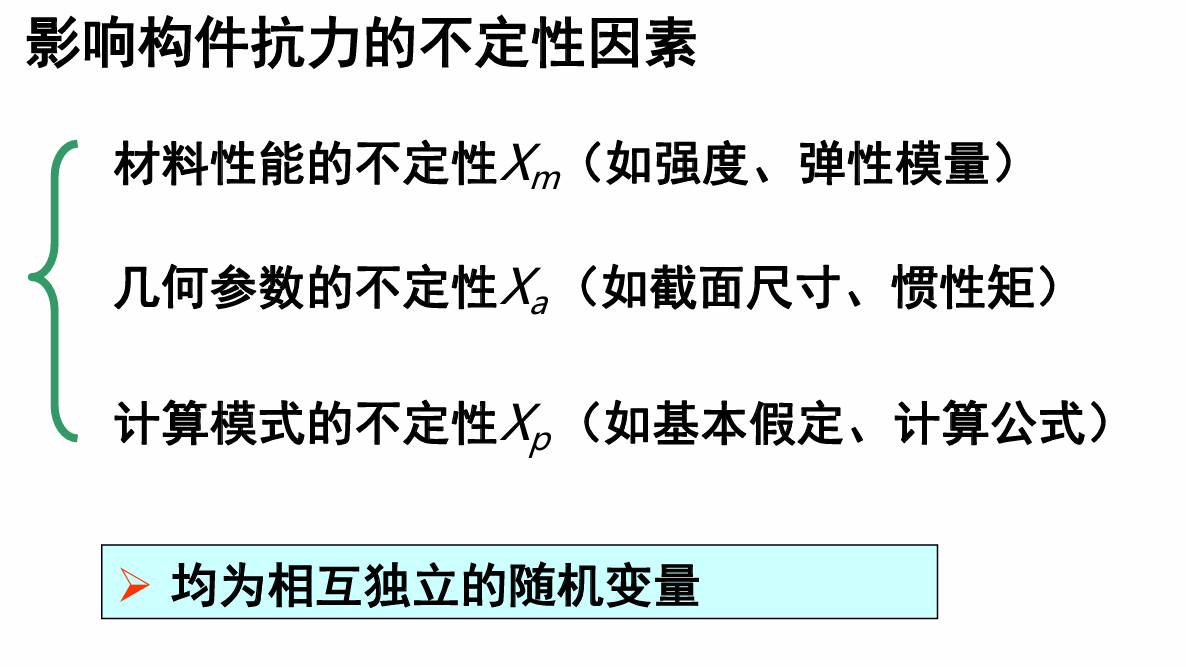
\includegraphics[width=0.7\textwidth]{../figure/yxys.png}
    \caption{结构抗力影响因素}
    \label{fig:chap5:fig2}
\end{figure}

\begin{theorem}
    若随机变量序列\(X_1, X_2, \ldots, X_n\)中的任何一个都不占优势,当\(n\)充分大时,无论\(X_1, X_2, \ldots, X_n\)具有怎样的分布,只要它们相互独立,若\(Y = \prod_{i=1}^{n} X_i\),则\(\ln Y = \sum_{i=1}^{n} \ln X_i\)趋近于正态分布,而\(Y\)近似服从对数正态分布。
\end{theorem}

\section{结构可靠度统计}

\begin{definition}
    结构可靠度是结构可靠性的概率量度(实际上不论如何设计,都无法确保百分百$R\le S$)

    更科学的定义是,结构在规定的时间内,在规定的条件下,完成预定功能的概率。
\end{definition}

\begin{definition}
    \[ Z = g(R, S) = R - S \quad \text{(9-1)} \]
上式称为结构功能函数,式中R, S均为随机变量,因此Z也是一个随机变量,总可能出现以下三种情况:
\[ Z > 0 \quad \text{结构可靠} \]
\[ Z < 0 \quad \text{结构失效} \]
\[ Z = 0 \quad \text{结构处于极限状态} \]
\end{definition}

(1)承载能力极限状态,对应于结构或结构构件达到最大承载能力或不适于继续承载的变形。

举例:结构或部分结构作为刚体失去平衡(如倾覆);结构构件或连接因材料强度被超过而破坏(如疲劳破坏)或因过渡到塑性变形而不适于继续承载;结构转变为机动体系;结构或结构构件丧失稳定(如压屈)

(2)正常使用极限状态,对应于结构或结构构件达到正常使用的某项规定限值。

举例:影响正常使用或外观的变形;影响正常使用的局部破坏;影响正常使用的振动;影响正常使用的其他特定状态。

(3)耐久性极限状态,对应于结构或结构构件达到耐久性能的某项规定限值。

举例:影响承载能力和正常使用的材料性能劣化;影响耐久性能的裂缝、变形、缺口、外观、材料削弱等;影响耐久性能的其他特定状态。

\section{中心点法}

\begin{definition}
    结构功能函数为线性函数情况(非线性的情况直接泰勒展开)

    设结构功能函数具有如下形式:
\[ Z = a_0 + \sum_{i=1}^{n} a_i X_i  \]
式中 \( a_0, a_i (i = 1, 2, \ldots, n) \) 
求得功能函数的均值和均方差分别为:
\[ \mu_Z = a_0 + \sum_{i=1}^{n} a_i \mu_{X_i}  \]
\[ \sigma_Z = \sqrt{\sum_{i=1}^{n} (a_i \sigma_{X_i})^2}  \]
式中 \(\mu_{X_i}, \sigma_{X_i}\) 是 \(X_i\) 的均值和均方差。
\end{definition}

解释下,这里的假设是,$R$和$S$都是对数正态分布的随机变量(具有合理性,因为大量正态分布随机变量的乘积近似服从对数正态分布),因此$Z$也是对数正态分布的随机变量。

我们设$\beta$为可靠指标,$\beta = \frac{\mu_Z}{\sigma_Z}$,在已知失效概率$p_f$情况下,可靠指标$\beta$与失效概率$p_f$的关系为:
\[
p_f = P(Y \leq \beta) = \Phi(-\beta)
\]
    式中 \(\Phi\) 是标准正态分布函数。
\begin{remark}
    可靠指标$\beta$越大,失效概率$p_f$越小,结构可靠度越高。

    可靠指标$\beta$的值通常在1.5到3.0之间。
    可靠指标$\beta$的值越大,结构的安全裕度越大。
\end{remark}

\begin{remark}
    可靠指标的几何含义为:当$X_1, X_2, \ldots, X_n$为独立正态随机向量时,且极限状态
曲面为线性曲面,则在其标准化空间中,原点到极限状态曲面的距
离为可靠指标的绝对值。
\end{remark}

\begin{example}
已知一伸臂梁如图 9-12 所示。梁所能承担的极限弯矩为 \( M_u \),若梁内弯矩 \( M > M_u \) 时,梁便失效。现已知各变量均服从正态分布,其各自的平均值及标准差为:荷载统计参数:\( \mu_p = 4 \text{kN} \),\( \sigma_p = 0.8 \text{kN} \);跨度统计参数:
\[
\mu_l = 6 \text{m}, \sigma_l = 0.1 \text{m} \text{;极限弯矩统计参数:} \mu_{M_u} = 20 \text{kN} \cdot \text{m}, \sigma_{M_u} = 2 \text{kN} \cdot \text{m} \text{。}
\]
试用中心点法计算该构件的可靠指标 \( \beta \)。

\begin{figure}[H]
\centering
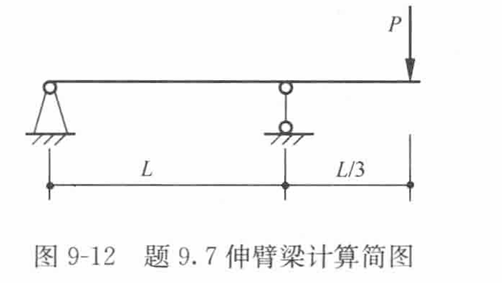
\includegraphics[width=0.6\textwidth]{../figure/5.png}
\end{figure}

\[
Z = M_u - \frac{1}{3} P l
\]
\[
\begin{cases}
F_1 + F_2 = P \\
F_1 l + P \cdot \frac{l}{3} = 0
\end{cases}
\]
\[
F_1 = -\frac{1}{3} P, \quad F_2 = \frac{4}{3} P
\]
\[
\mu_Z = \mu_{Mu} - \frac{1}{3} \mu_P \mu_l = 20 - \frac{1}{3} \times 4 \times 6 = 12 \text{ kN} \cdot \text{m}
\]
偏导数计算:
\[
\frac{\partial Z}{\partial M_u} = 1, \quad \frac{\partial Z}{\partial P} =-\frac{1}{3} l, \quad \frac{\partial Z}{\partial l} = -\frac{1}{3} P
\]
标准差计算:
\[
\sigma_Z = \sqrt{
    (\sigma_{M_u})^2 + \left(\frac{1}{3} \mu_l \sigma_ P \right)^2 + \left(\frac{1}{3} \mu_P \sigma_l \right)^2
} 
= 2.56
\]
计算系数 $\beta$:
\[
\beta = \frac{\sigma_Z}{M_Z} = \frac{2.56}{12} = 0.213
\]
\end{example}

\ifx\allfiles\undefined
\end{document}
\fi